\chapter{Prise de mesures}
Ce chapitre traite de la collecte des données qui est un point important de ce travail. Il a été nécessaire de réfléchir à quoi prendre et de quelle manière. Pour ce faire, je me suis servi d'un système de mesures de positionnement intérieur développé par M. Mueller dans le cadre de son travail de Master \cite{MIC}. Ci-dessous, ce programme sera détaillé plus précisément afin de pouvoir le prendre en main et réaliser les prises de mesures. 

Il sera également précisé comment les données ont été structurées afin de pouvoir être utilisée plus tard pour alimenter l'algorithme d'apprentissage. 

Finalement, il sera détaillé comment les mesures ont été effectuées selon le plan du laboratoire.

\section{Plan de mesure}
Un plan de mesure idéal avait été imaginé dans un premier temps pour effectuer les premiers essais, voir sur la Figure \ref{fig:PlanMod}. Ce plan n'a pas pu être réalisé exactement de cette manière dû à la configuration de la salle et de la disposition des établis. Comme décrit ci-dessus, la configuration de la salle pour effectuer les mesures est composée de quatre esclaves (Slaves) placés dans les coins de la pièce à mesurer et le maitre (master) est placé au centre. Ensuite, l'espion est déplacé à différents endroits pour effectuer la prise de mesures voir sur la Figure \ref{fig:mesures}.

\begin{figure}[htp]
 \begin{center}
  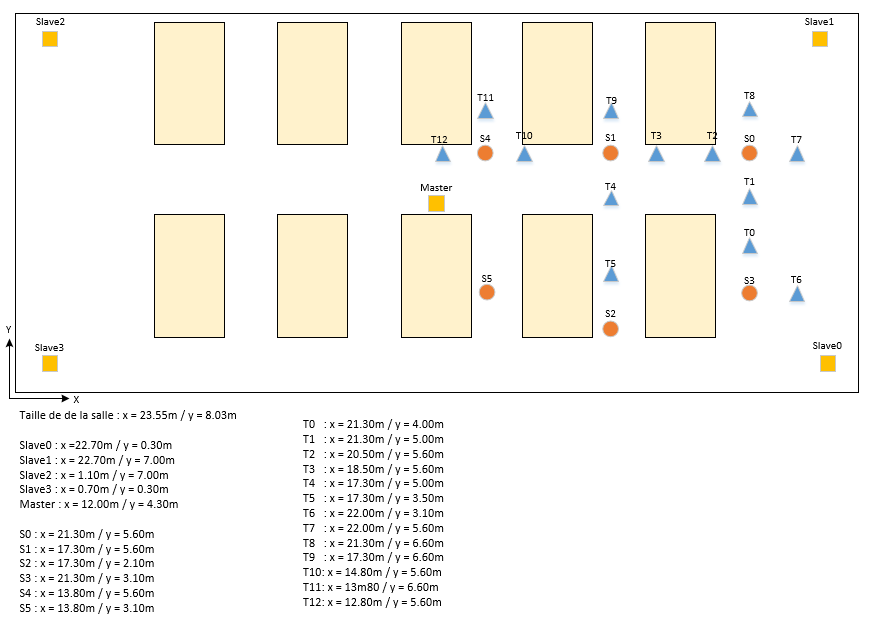
\includegraphics[scale=0.7]{figures/mesures.png}
  \caption{Plan des mesures effectuées et du setup}
  \label{fig:mesures} %% NOTE: always label *after* caption!
 \end{center}
\end{figure}

Afin de mieux comprendre la méthodologie de mesures, un cas réel a été imaginé. C'est-à-dire, que la réflexion a été faite en partant du principe qu'il faut positionner des objets dans un laboratoire et installer le système sans effectuer un quadrillage trop précis afin que le temps d'action soit le plus court possible. 

Les points marqués par Sx (orange foncé) sont les points sur lesquels le système est basé et correspondent à la position de l'espion (spy). Quarante mesures ont été effectuées sur ces six endroits et c'est eux qui seront utilisés pour entrainer le système. Cinq mesures supplémentaires ont été effectuées à ces endroits pour les vérifications. Ces mesures ont été effectuées à des moments différents à l'exception de S5.

Les triangles bleus marqués Tx correspondent à des points de tests et cinq mesures ont été effectuées par point. 

À noter que toutes ces mesures ont été effectuées en positionnant un mat muni d'un carton pour poser la carte de l'espion. Donc à chaque changement de position, il est possible que cette dernière varie de quelques centimètres et que l'orientation de l'antenne soit différente. 

\section{Setup pour la prise de mesures}
Pour effectuer les prises de position, il est nécessaire d'effectuer un certain nombre de mesures afin d'avoir une quantité acceptable de données. Dans un premier temps, l'idée est de se concentrer sur le plan du laboratoire. Pour une première version d'apprentissage, les mesures seront effectuées dans une seule moitié du laboratoire comme indiqué sur la Figure \ref{fig:PlanMod}.

Le point rond "M" représente le maitre, les points ronds "S" représentent les esclaves et finalement les points carrés "E" représentent les espions. C'est sur ces derniers que les mesures seront effectuées. 

Il sera nécessaire de prendre quarante mesures sur chaque point. Comme uniquement la première moitié sera considéré, les mesures seront faites sur six points différents donc 240 données seront à disposition. Une mesure consiste à changer les canaux de 1 à 40.

\begin{figure}[htp]
 \begin{center}
  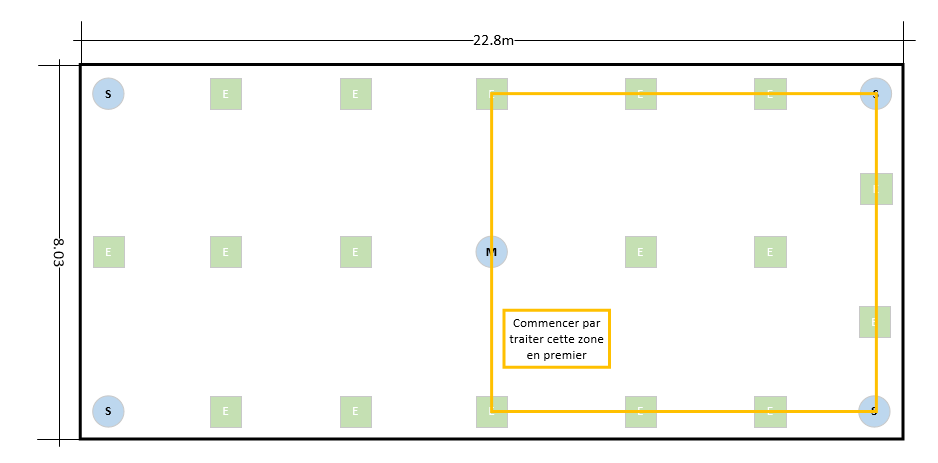
\includegraphics[scale=0.5]{figures/PlanMod.PNG}
  \caption{Montre le setup pour la prise de mesure}
  \label{fig:PlanMod} %% NOTE: always label *after* caption!
 \end{center}
\end{figure}

Le plan de la Figure \ref{fig:PlanMod} et une simplification du plan réel de la Figure \ref{fig:PlanRe}.

\begin{figure}[htp]
 \begin{center}
  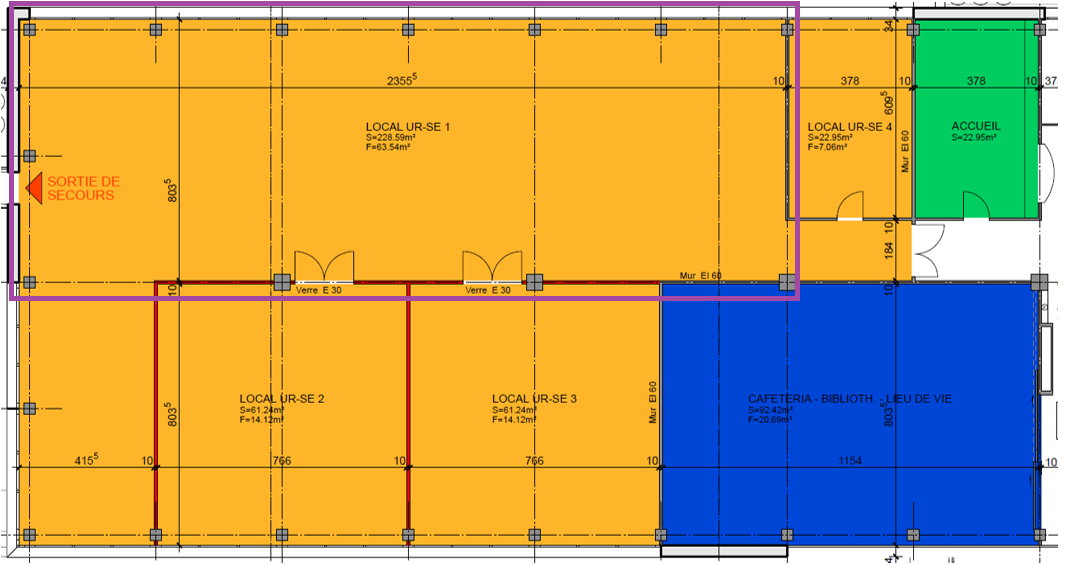
\includegraphics[scale=0.5]{figures/PlanRe.PNG}
  \caption{Montre le plan réel du laboratoire}
  \label{fig:PlanRe} %% NOTE: always label *after* caption!
 \end{center}
\end{figure}

\subsection{Matériel utilisé}
Les cartes utilisées durant ce travail pour les noeuds du système de mesures sont présentées dans la Figure \ref{fig:carte}. Les noeuds sont : les quatre esclaves, le maitre et l'espion. La carte provient de chez Semtech et utilise la radio SX1280, elle est interfacée sur une carte Nucleo-F410RB de chez STMicroelectronics.
 
\begin{figure}[htp]
 \begin{center}
  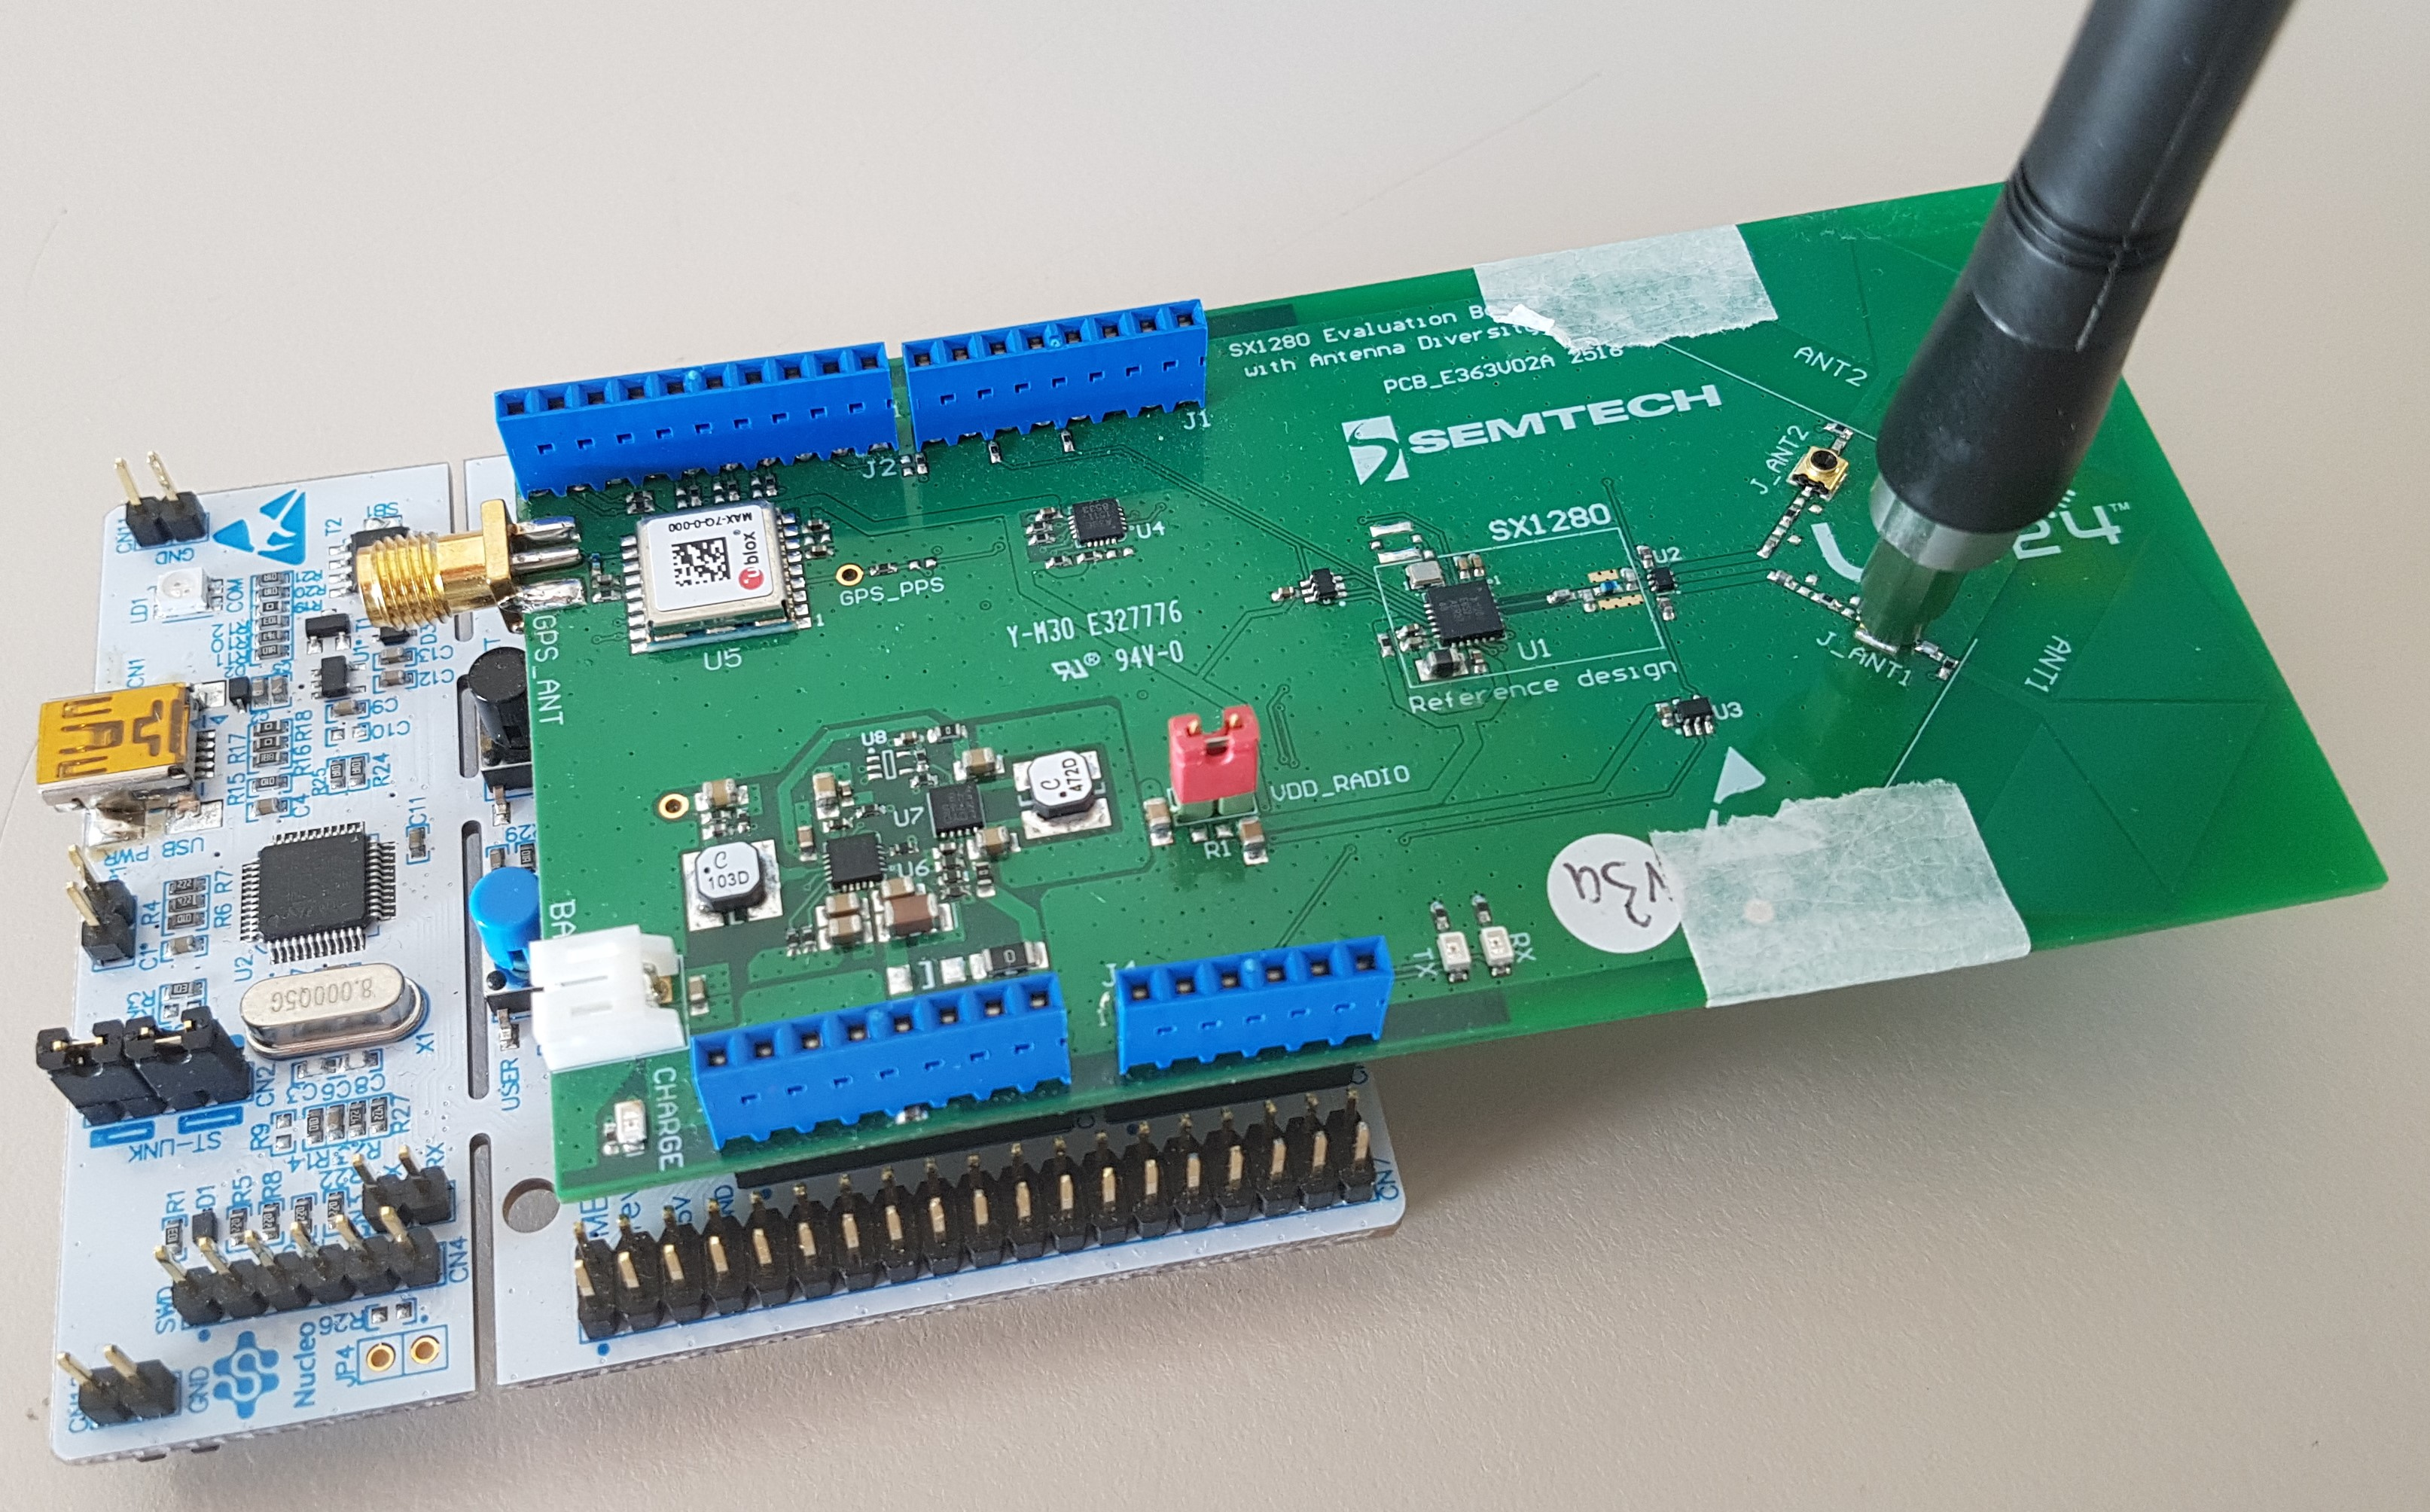
\includegraphics[scale=0.1]{figures/carte.jpg}
  \caption{Montre le plan réel du laboratoire}
  \label{fig:carte} %% NOTE: always label *after* caption!
 \end{center}
\end{figure}

Chaque carte est configurée séparément pour fonctionner selon sa fonction (esclave, maitre ou espion). Il suffit de connecter la carte à un ordinateur et de glisser dans le répertoire qui s'ouvre le fichier "image" correspondant à la fonctionnalité. 

\section{Programme de prise de mesure \cite{MIC}}

Cette section introduit le programme de prise de mesure qui avait été développé. Ce programme permet avant tout d’exploiter pleinement le protocole de localisation, ainsi que les algorithmes de résolution de position. 

Le système peut être composé d’un ou plusieurs esclaves et d’un ou plusieurs maîtres. Les espions font bien entendu partie intégrante également. Le programme effectue des mesures de distance, résout des positions des différents espions et les affiche dans une interface graphique. Le tout est configurable au travers d’un simple fichier de configuration au format texte.

Dans le cadre de ce projet, le fichier de configuration (stage.cfg) contient les informations (position, id,etc.) du "maitre" ainsi que des quatre esclaves. 

Le programme réalisé pour ce démonstrateur a dû être adapté, car il a été conçu pour effectuer des mesures en continu afin d'améliorer au fil du temps le calcul de la position. Cette façon de faire n'est pas utilisable dans le cadre d'un apprentissage à l'aide d'un algorithme.

\subsection{Architecture logicielle}
Pour avoir une meilleure compréhension la structure du programme de prise de mesures, la Figure \ref{fig:archLR24} permet de visualiser les blocs principaux qui interagissent dans le calcul de position.

\begin{figure}[htp]
 \begin{center}
  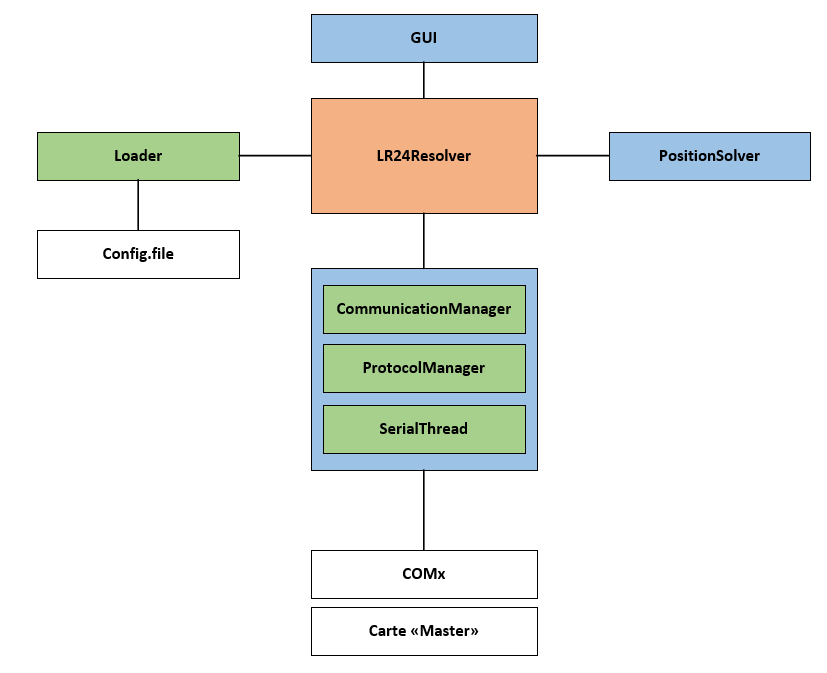
\includegraphics[scale=0.7]{figures/architecture_LR24.PNG}
  \caption{Blocs principaux du logiciel de prise de mesure}
  \label{fig:archLR24} %% NOTE: always label *after* caption!
 \end{center}
\end{figure}

Ci-dessous, une description de chaque bloc est présentée :

\begin{enumerate}
 \item LR24Resolver : Partie centrale du démonstrateur (chef d’orchestre). Il instancie les autres blocs et gère les différents bursts de mesure et de communication).
 \item Loader : Chargé de lire le fichier de configuration et de créer un jeu d’objets utilisables facilement par les autres blocs.
 \item GUI : Interface graphique du système. Il affiche la position des maîtres (carrés verts), des esclaves (cercles verts), des espions (cercles jaunes) et les distances maître-esclave (cercles rouges).
 \item PostionSolver : Chargé de résoudre la position des espions en se basant sur leurs mesures. Il utilise la méthode d’approximation aux moindres carrés avancés.
 \item SerialThread : Communication avec la carte embarquée de type maître. Ce bloc utilise le port série standard. Il lit les données disponibles et les remontes à la couche supérieure. Il transmet aussi les bytes reçus de la couche supérieure vers le port série.
 \item ProtocolManager : Gestion du format du protocole de communication. Cela signifie qu’il transforme les trames reçues en jeu d’objets utilisables, ou alors, il transforme des objets reçus en une trame valide.
 \item CommunicationManager : Gestion des actions (mesure, communication, calibration, etc.). Il reçoit des actions et les exécute au travers du "ProtocolManager".
\end{enumerate}

Une interface graphique est disponible avec le programme lors du lancement. Il est possible de démarrer une mesure, de l'interrompre et de la remettre à zéro, Figure \ref{fig:GUI_LR24}.

\begin{figure}[htp]
 \begin{center}
  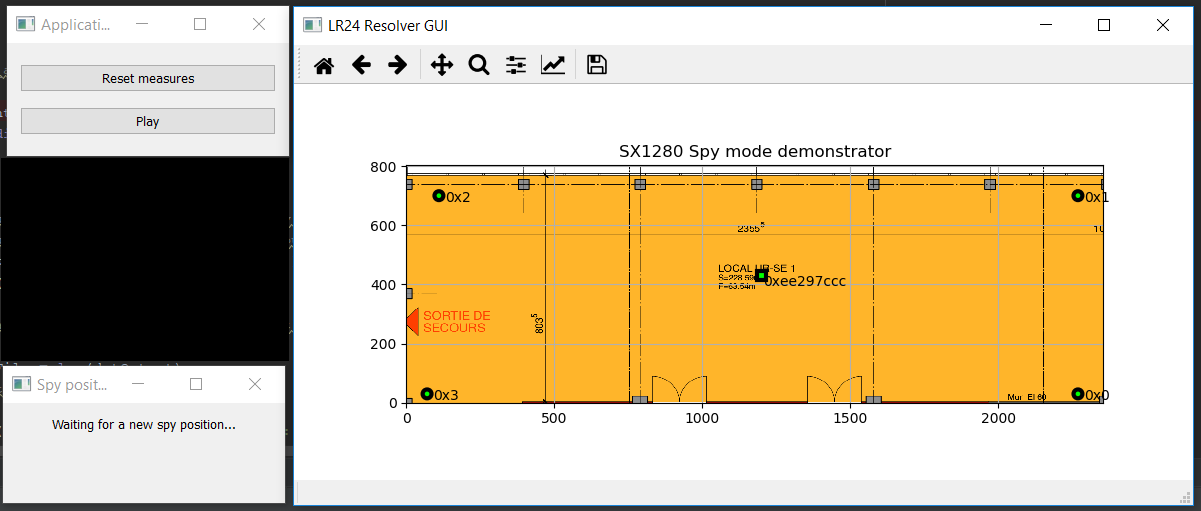
\includegraphics[scale=0.7]{figures/LR24_GUI.png}
  \caption{Interface graphique du soft de prise de mesures}
  \label{fig:GUI_LR24} %% NOTE: always label *after* caption!
 \end{center}
\end{figure}

Ce programme est fait pour ordonner à la carte embarquée "maitre" d'effectuer une série de mesures. Ensuite, dès que le maitre reçoit une mesure de l'espion, il la transfère au programme qui tourne sur le PC. Les mesures réceptionnées sont sous forme de burst. Les informations utiles de ces bursts sont : 

\begin{enumerate}
 \item La provenance du burst de mesure (mesure effectuée sur quel esclave?)
 \item La mesure brute de différence de distance pour chaque esclave et pour quarante canaux de fréquence différents.
 \item La mesure brute du RSSI 
\end{enumerate}

La position de l'espion est calculée au niveau du programme PC (PositionSolver) en fonction des données reçues vu précédemment. Selon le fichier de configuration, les mesures sont faites sur plusieurs canaux (ranging slot number = 40). Le système va effectuer les étapes suivantes en boucle en mesurant séquentiellement chaque esclave: 

\begin{enumerate}
 \item Mesure sur 40 canaux sur un esclave
 \item Récupérer les données sur les maitres
 \item Transmettre les données au niveau du PC
 \item Mesurer le deuxième esclave
 \item Récupérer les données sur le master
 \item Estimation de position quand cela est possible
\end{enumerate}

La fonction qui réceptionne les burst entrant et par conséquent la structure des données se trouve dans le callback ci-dessous :

\begin{lstlisting}
def new burst available(burst_list) :
'''
Callback when new bursts are available
:param burst_list: list_of_bursts
:return: None

=> It will calculate nodes new positions
'''
for burst in burst list:
position solver.update position_solver(burst)
system_gui.update_burst_info(burst)
\end{lstlisting}

Ce callback est reçu dans lr24\_resolver.py. C'est une liste de burst (en python). En résumé, les burst reçus stock toutes les mesures pour un couple maitre-esclave :

valeurs[0, canal] = mesure brute pour un canal donné\.\\
valeurs[1, canal] = rssi pour un canal donné\.\\
valeurs[2, canal] = erreur pour un canal\.\\

Ces données doivent être exploiter pour la suite du travail. 

\subsection{Prise de données brutes}
La prise de données brutes consiste à mémoriser les valeurs brutes des informations de différences de distance fournie par l'espion. Cette mesure provient du fonctionnement des cartes embarquées qui sont configurées pour fonctionner en mode espion. Cette donnée se calcule en faisant Mspy = D1+D2-D3, voir Figure \ref{fig:mesures3}. Lorsque le système possède quatre esclaves, il y aura une mesure par esclave sur chaque fois les quarante canaux. C'est avec ces dernières qu'une position est estimée. 

\begin{figure}[htp]
 \begin{center}
  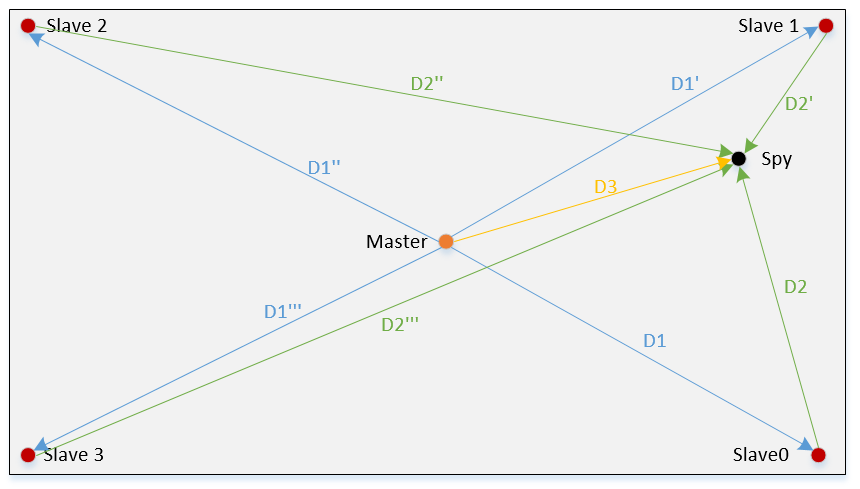
\includegraphics[scale=0.7]{figures/mesures3.png}
  \caption{Fonctionnement du mode spy et signification des mesures brutes}
  \label{fig:mesures3} %% NOTE: always label *after* caption!
 \end{center}
\end{figure}
 
\subsubsection{Modification du programme lr24\_resolver.py}
Le programme Lr24\_resolver.py n'a pas pu être utilisé de la manière dont il avait été créé, car il était destiné à effectuer des mesures continues afin d'améliorer au fil du temps la précision. Dans le cadre de ce projet, il est nécessaire de pouvoir maitriser la prise de mesures ainsi que gérer le nombre d'échantillons enregistrés. La Figure \ref{fig:mesures} montre de quelle manière sont prises les données.

Il a été nécessaire de modifier la fonction new\_burst\_available(burst\_list) du fichier Lr24\_resolver.py afin de mémoriser les huit premiers burst qui arrivent depuis la carte "maitre". De ces "burst" sera uniquement mémorisée la valeur de la différence de distance calculée par l'espion. Cette différence de distance est obtenue grâce au mode "ranging" de la communication LoRa. Un "burst" comprend quarante informations qui sont liées aux quarante canaux de mesures. 

Une fois que les huit bursts ont été reçus, le calcul de position, s’il existe, est mémorisé puis remis à zéro pour la mesure suivante. Il est possible de sélectionner le nombre de mesures désirées grâce à la variable "measures\_count\_des". Quand ce nombre est atteint, le programme s'arrête automatiquement, sinon il continue d'effectuer les mesures.

La fonction "new\_node\_position\_available(node\_pos)" a également été adaptée. Lorsqu'une mesure de position existe, il y a un contrôle qui est effectué afin de s'assurer que les mesures ont été effectuées dans un ordre précis qui est le suivant : Burst reçu de la mesure sur le slave0 (2x) puis du slave1 (2x) puis du slave2 (2x) et finalement du slave3 (2x). Cela afin de ne pas mélanger les données lors de l'apprentissage à l'aide de l'algorithme SVM. 

Finalement, pour que les mesures soient automatiques avec le moins d'interaction possible avec l'utilisateur le fichier gui.py a été modifié pour y ajouter les fonctions software des boutons "stop", "start" et "reset". 

\begin{figure}[htp]
 \begin{center}
  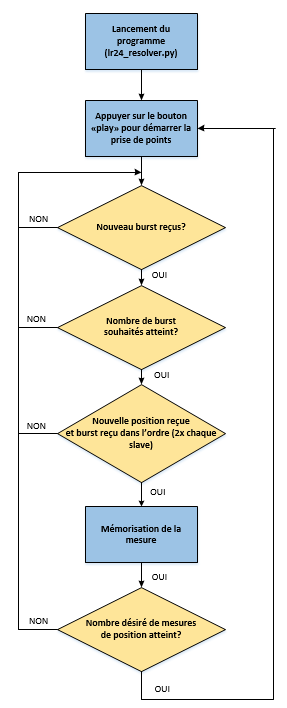
\includegraphics[scale=0.7]{figures/PriseMesures.png}
  \caption{Diagramme expliquant la prise de mesures des valeurs de ranging}
  \label{fig:mesures} %% NOTE: always label *after* caption!
 \end{center}
\end{figure}

\subsubsection{Structure des données}

Dans la Figure \ref{fig:dataStruct} est représenté comment sont structurées les mesures récupérées par le programme python (Lr24\_resolver.py). Il a été nécessaire de faire une réflexion concernant quoi prendre comme mesure et de quelle manière. Il a été décidé de récupérer les informations ci-dessous. A noter qu'un fichier est créé par endroit de mesure, c'est-à-dire qu'a chaque changement de position un nouveau fichier est construit.

\begin{enumerate}
 \item Index : Numéro de la mesure pour un point donné
 \item X1 : Coordonnée X réelle par rapport aux repères de la salle 
 \item Y1 : Coordonnée Y réelle par rapport aux repères de la salle 
 \item X2 : Coordonnée X calculée par le programme python Lr24\_resolver.py après avoir reçus huit bursts
 \item Y2 : Coordonnée Y calculée par le programme python Lr24\_resolver.py après avoir reçus huit bursts
 \item meas : Données brutes de la valeur de "ranging" sur les quarante canaux reçues à chaque burst (8x40 valeurs)
\end{enumerate}

Une décision a été prise à ce niveau de ne pas utiliser le RSSI. Effectivement, la prise de mesures est plus complexe qu'espérée et prend passablement de temps. Le RSSI aurait pu être intégré par la suite en pensant qu'une mesure était rapidement faite, mais ce n'a pas été le cas. 

Sur la Figure \ref{fig:dataStruct} la partie "meas" est séparée en quatre parties, car les bursts sont reçus dans l'ordre deux fois pour l'esclave 0, deux fois pour l'esclave 1, deux fois pour l'esclave 2 et finalement deux fois pour l'esclave 3. 

\begin{figure}[htp]
 \begin{center}
  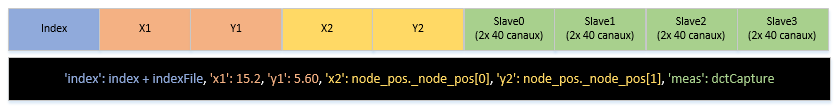
\includegraphics[scale=0.7]{figures/dataStruct.png}
  \caption{Structure des données des mesures de localisation}
  \label{fig:dataStruct} %% NOTE: always label *after* caption!
 \end{center}
\end{figure}

\subsection{Prise de données de positions convergées}
La prise de données des positions convergées est similaire à la prise des mesures brutes sauf que lors du lancement de la mesure, il faut laisser la mesure converger sur sa position finale et la mémoriser sans tenir compte des valeurs brutes des différents canaux.

Cette prise de mesure supplémentaire a été réalisée, car les résultats obtenus uniquement avec les valeurs brutes ne sont pas complétement satisfaisants (voir dans le chapitre suivant). 

\subsubsection{Modification du programme lr24\_resolver.py}
Pareil que ci-dessus, le programme Lr24\_resolver.py n'a pas pu être utilisé comme il avait été créé, car il était destiné à effectuer des mesures continues afin d'améliorer au fil du temps la précision. Dans le cadre de ce projet, il est nécessaire de pouvoir maitriser la prise de mesures. La Figure \ref{fig:mesures2} montre de quelle manière sont prises les données de positions convergées.

Les modifications apportées au logiciel sont similaires à celles détaillées ci-dessus. La seule différence c'est qu'il a été nécessaire de regarder à partir de quel moment la mesure converge et effectuer ce nombre de mesures pour chaque point. La mesure dure environ trois minutes pour obtenir une position convergée ce qui correspond à la réception de 120 burst. 

Le résultat de la position est mémorisé à la suite des 120 burst. 

\begin{figure}[htp]
 \begin{center}
  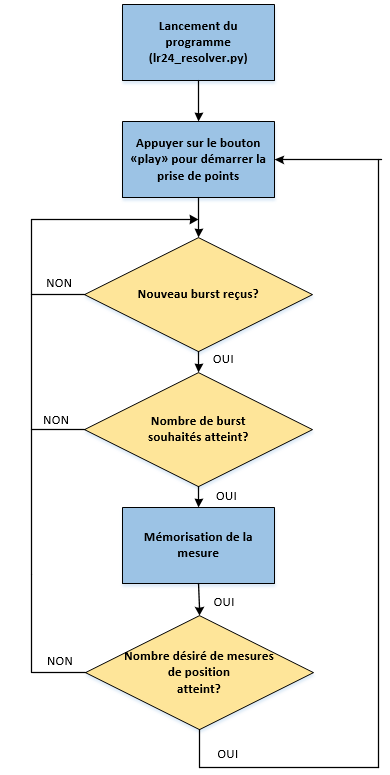
\includegraphics[scale=0.7]{figures/PriseMesures2.png}
  \caption{Diagramme expliquant la prise de mesures des positions convergées}
  \label{fig:mesures2} %% NOTE: always label *after* caption!
 \end{center}
\end{figure}

\subsubsection{Structure des données}
La structure des données voir la Figure \ref{fig:dataStruct2} est similaire à la partie ci-dessus sauf que les données brutes ne sont pas mémorisées, car leur nombre serait trop important. 

\begin{enumerate}
 \item Index : Numéro de la mesure pour un point donné
 \item X1 : Coordonnée X réelle par rapport aux repères de la salle 
 \item Y1 : Coordonnée Y réelle par rapport aux repères de la salle 
 \item X2 : Coordonnée X calculée par le programme python Lr24\_resolver.py après avoir convergée (120 bursts)
 \item Y2 : Coordonnée Y calculée par le programme python Lr24\_resolver.py après avoir convergée (120 bursts)
\end{enumerate}

\begin{figure}[htp]
 \begin{center}
  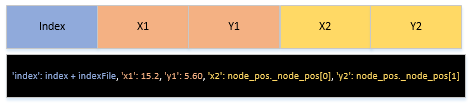
\includegraphics[scale=0.7]{figures/dataStruct2.png}
  \caption{Structure des données de mesures contenant uniquement la valeur des positions convergées}
  \label{fig:dataStruct2} %% NOTE: always label *after* caption!
 \end{center}
\end{figure}



%\begin{lstlisting}
% for i=0 to Array.length(t)-1 do
%\end{lstlisting}


%\begin{enumerate}
% \item fgfd
% \item gdgfd
%\end{enumerate}


%\begin{figure}[H]
% \begin{center}
%  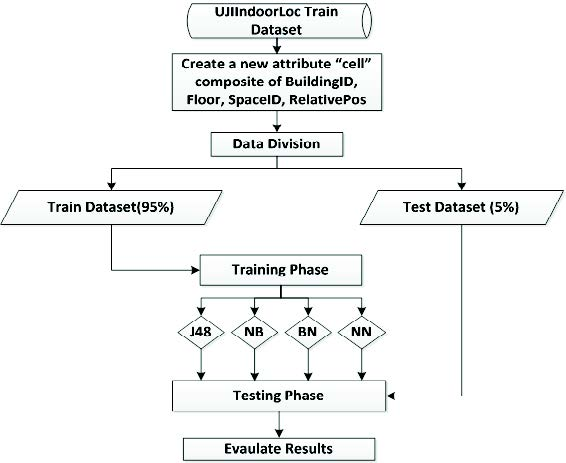
\includegraphics[scale=1]{figures/newattribute.jpg}
%  \caption{The new attribute “cell” construction phase}
%  \label{fig:newAttribute} %% NOTE: always label *after* caption!
% \end{center}
%\end{figure}

%\todo{Compléter cette partie qui semble importante}

